% answers.tex —— 2009 年·全国大纲卷Ⅰ·理科 · 参考答案与详细解析片段
% 由 tools/generate_projects.py 依来源总账自 2009/2009_数学真题_全国1理_试题.md + 2009/2009_数学真题_全国1理_解析正文.md + 2009/2009_数学真题_全国1理_答案要点.md 生成，勿手改（改源 MD 后重跑）


\begin{gktip}
固定源 PDF 为印刷页码 507–508 的两页题面，不附答案。以下解析均依据固定源独立复算；第 18、21、22 题图形在 LaTeX 工程中以 TikZ/PGFPlots 矢量源重绘。
\end{gktip}

\begin{answer}
\gksolhead{1}{}

\textbf{题目}：

设集合 $A=\{4,5,7,9\}$，$B=\{3,4,7,8,9\}$，全集 $U=A\cup B$，则集合 $\complement_U(A\cap B)$ 中的元素共有\mbox{（　　）}

（A）$3$ 个\quad（B）$4$ 个\quad（C）$5$ 个\quad（D）$6$ 个

\Needspace{4\baselineskip}
\textbf{解析}

$A\cap B=\{4,7,9\}$，$U=\{3,4,5,7,8,9\}$，所以补集为
$\{3,5,8\}$，选 A。

\gkanswer{答案：A}

\end{answer}
\begin{answer}
\gksolhead{2}{}

\textbf{题目}：

已知 $\dfrac{\overline z}{1+i}=2+i$，则复数 $z=$\mbox{（　　）}

（A）$-1+3i$\quad（B）$1-3i$\quad（C）$3+i$\quad（D）$3-i$

\Needspace{4\baselineskip}
\textbf{解析}

由 $\overline z=(2+i)(1+i)=1+3i$，故 $z=1-3i$，选 B。

\gkanswer{答案：B}

\end{answer}
\begin{answer}
\gksolhead{3}{}

\textbf{题目}：

不等式 $\left|\dfrac{x+1}{x-1}\right|<1$ 的解集为\mbox{（　　）}

（A）$\{x\mid0<x<1\}\cup\{x\mid x>1\}$\quad（B）$\{x\mid0<x<1\}$\quad（C）$\{x\mid-1<x<0\}$\quad（D）$\{x\mid x<0\}$

\Needspace{4\baselineskip}
\textbf{解析}

\nopagebreak[4]
\[
\left|\frac{x+1}{x-1}\right|<1
\Longleftrightarrow (x+1)^2<(x-1)^2
\Longleftrightarrow x<0,
\]

故选 D。

\gkanswer{答案：D}

\end{answer}
\begin{answer}
\gksolhead{4}{}

\textbf{题目}：

设双曲线 $\dfrac{x^2}{a^2}-\dfrac{y^2}{b^2}=1$（$a>0,b>0$）的渐近线与抛物线 $y=x^2+1$ 相切，则该双曲线的离心率等于\mbox{（　　）}

（A）$\sqrt3$\quad（B）$2$\quad（C）$\sqrt5$\quad（D）$\sqrt6$

\Needspace{4\baselineskip}
\textbf{解析}

渐近线与抛物线相切给出 $\dfrac ba=2$，所以
$e=\sqrt{1+b^2/a^2}=\sqrt5$，选 C。

\gkanswer{答案：C}

\end{answer}
\begin{answer}
\gksolhead{5}{}

\textbf{题目}：

甲组有 $5$ 名男同学、$3$ 名女同学；乙组有 $6$ 名男同学、$2$ 名女同学。若从甲、乙两组中各选出 $2$ 名同学，则选出的 $4$ 人中恰有 $1$ 名女同学的不同选法共有\mbox{（　　）}

（A）$150$ 种\quad（B）$180$ 种\quad（C）$300$ 种\quad（D）$345$ 种

\Needspace{4\baselineskip}
\textbf{解析}

\Needspace{5\baselineskip}
与文科卷同样分类计数：

\nopagebreak[4]
\[
\binom31\binom51\binom62+\binom52\binom21\binom61
=345,
\]

故选 D。

\gkanswer{答案：D}

\end{answer}
\begin{answer}
\gksolhead{6}{}

\textbf{题目}：

设 $\boldsymbol a\text{、}\boldsymbol b\text{、}\boldsymbol c$ 是单位向量，且 $\boldsymbol a\cdot\boldsymbol b=0$，则 $(\boldsymbol a-\boldsymbol c)\cdot(\boldsymbol b-\boldsymbol c)$ 的最小值为\mbox{（　　）}

（A）$-2$\quad（B）$\sqrt2-2$\quad（C）$-1$\quad（D）$1-\sqrt2$

\Needspace{4\baselineskip}
\textbf{解析}

\nopagebreak[4]
\[
(\boldsymbol a-\boldsymbol c)\cdot(\boldsymbol b-\boldsymbol c)
=1-\boldsymbol c\cdot(\boldsymbol a+\boldsymbol b).
\]

因 $\boldsymbol a\perp\boldsymbol b$ 且均为单位向量，
$|\boldsymbol a+\boldsymbol b|=\sqrt2$。柯西不等式给出最小值
$1-\sqrt2$，选 D。

\gkanswer{答案：D}

\end{answer}
\begin{answer}
\gksolhead{7}{}

\textbf{题目}：

已知三棱柱 $ABC-A_1B_1C_1$ 的侧棱与底面边长都相等，$A_1$ 在底面 $ABC$ 上的射影为 $BC$ 的中点，则异面直线 $AB$ 与 $CC_1$ 所成的角的余弦值为\mbox{（　　）}

（A）$\dfrac{\sqrt3}{4}$\quad（B）$\dfrac{\sqrt5}{4}$\quad（C）$\dfrac{\sqrt7}{4}$\quad（D）$\dfrac34$

\Needspace{4\baselineskip}
\textbf{解析}

底面为边长 $2$ 的正三角形，$A_1$ 到 $BC$ 中点的水平距离为
$\sqrt3$，而侧棱长为 $2$，故其竖直分量为 $1$。计算
$\overrightarrow{AB}\cdot\overrightarrow{CC_1}=3$，两向量长均为 $2$，
所以余弦为 $\dfrac34$，选 D。

\gkanswer{答案：D}

\end{answer}
\begin{answer}
\gksolhead{8}{}

\textbf{题目}：

如果函数 $y=3\cos(2x+\varphi)$ 的图象关于点 $\left(\dfrac{4\pi}{3},0\right)$ 中心对称，那么 $|\varphi|$ 的最小值为\mbox{（　　）}

（A）$\dfrac\pi6$\quad（B）$\dfrac\pi4$\quad（C）$\dfrac\pi3$\quad（D）$\dfrac\pi2$

\Needspace{4\baselineskip}
\textbf{解析}

中心对称点满足 $2x+\varphi=\dfrac\pi2+k\pi$。代入
$x=\dfrac{4\pi}{3}$ 后，$\varphi$ 的最小绝对值为 $\dfrac\pi6$，选 A。

\gkanswer{答案：A}

\end{answer}
\begin{answer}
\gksolhead{9}{}

\textbf{题目}：

已知直线 $y=x+1$ 与曲线 $y=\ln(x+a)$ 相切，则 $a$ 的值为\mbox{（　　）}

（A）$1$\quad（B）$2$\quad（C）$-1$\quad（D）$-2$

\Needspace{4\baselineskip}
\textbf{解析}

\Needspace{5\baselineskip}
相切点 $(x,y)$ 满足

\nopagebreak[4]
\[
y=x+1=\ln(x+a),\qquad \frac1{x+a}=1.
\]

故 $x+a=1$ 且 $x+1=0$，得到 $x=-1,a=2$，选 B。

\gkanswer{答案：B}

\end{answer}
\begin{answer}
\gksolhead{10}{}

\textbf{题目}：

已知二面角 $\alpha-l-\beta$ 为 $60^\circ$，动点 $P\text{、}Q$ 分别在面 $\alpha\text{、}\beta$ 内，$P$ 到 $\beta$ 的距离为 $\sqrt3$，$Q$ 到 $\alpha$ 的距离为 $2\sqrt3$，则 $P\text{、}Q$ 两点之间距离的最小值为\mbox{（　　）}

（A）$\sqrt2$\quad（B）$2$\quad（C）$2\sqrt3$\quad（D）$4$

\Needspace{4\baselineskip}
\textbf{解析}

\Needspace{5\baselineskip}
与第 11 题同样在法截面内计算，两个点到棱的距离为 $2$ 和 $4$，故

\nopagebreak[4]
\[
PQ_{\min}=\sqrt{2^2+4^2-2\cdot2\cdot4\cos60^\circ}=2\sqrt3,
\]

选 C。

\gkanswer{答案：C}

\end{answer}
\begin{answer}
\gksolhead{11}{}

\textbf{题目}：

函数 $f(x)$ 的定义域为 $\mathbb R$，若 $f(x+1)$ 与 $f(x-1)$ 都是奇函数，则\mbox{（　　）}

（A）$f(x)$ 是偶函数\quad（B）$f(x)$ 是奇函数\quad（C）$f(x)=f(x+2)$\quad（D）$f(x+3)$ 是奇函数

\Needspace{4\baselineskip}
\textbf{解析}

\Needspace{5\baselineskip}
令 $g(x)=f(x+1)$，$h(x)=f(x-1)$。由 $g\text{、}h$ 均为奇函数：

\nopagebreak[4]
\[
f(1-x)=-f(1+x),\qquad f(-x-1)=-f(x-1).
\]

将第一式中的 $x$ 换为 $x+2$，可得
$f(x+3)=f(x-1)$。因此 $f(x+3)$ 与奇函数 $f(x-1)$ 相同，选 D。

\gkanswer{答案：D}

\end{answer}
\begin{answer}
\gksolhead{12}{}

\textbf{题目}：

已知椭圆 $C:\dfrac{x^2}{2}+y^2=1$ 的右焦点为 $F$，右准线为 $l$，点 $A\in l$，线段 $AF$ 交 $C$ 于点 $B$。若 $\overrightarrow{FA}=3\overrightarrow{FB}$，则 $|\overrightarrow{AF}|=$\mbox{（　　）}

（A）$\sqrt2$\quad（B）$2$\quad（C）$\sqrt3$\quad（D）$3$

\Needspace{4\baselineskip}
\textbf{解析}

右焦点 $F=(1,0)$、右准线 $x=2$。令 $A=(2,t)$，则
$B=(4/3,t/3)$，代入椭圆方程得 $t^2=1$，从而 $|AF|=\sqrt2$，选 A。

\gkanswer{答案：A}

\end{answer}
\begin{answer}
\gksolhead{13}{}

\textbf{题目}：

$(x-y)^{10}$ 的展开式中，$x^7y^3$ 的系数与 $x^3y^7$ 的系数之和等于\gkblank{}。

\Needspace{4\baselineskip}
\textbf{解析}

两个系数为 $-\binom{10}{3}$、$-\binom{10}{7}$，和为 $-240$。

\gkanswer{答案：$-240$}

\end{answer}
\begin{answer}
\gksolhead{14}{}

\textbf{题目}：

设等差数列 $\{a_n\}$ 的前 $n$ 项和为 $S_n$，若 $S_9=72$，则 $a_2+a_4+a_9=$\gkblank{}。

\Needspace{4\baselineskip}
\textbf{解析}

$S_9=72$ 给出 $a_1+a_9=16$，故
$a_2+a_4+a_9=\dfrac32(a_1+a_9)=24$。

\gkanswer{答案：$24$}

\end{answer}
\begin{answer}
\gksolhead{15}{}

\textbf{题目}：

直三棱柱 $ABC-A_1B_1C_1$ 的各顶点都在同一球面上。若 $AB=AC=AA_1=2$，$\angle BAC=120^\circ$，则此球的表面积等于\gkblank{}。

\Needspace{4\baselineskip}
\textbf{解析}

底面三角形的第三边
$BC=\sqrt{2^2+2^2-2\cdot2\cdot2\cos120^\circ}=2\sqrt3$，
\Needspace{5\baselineskip}
其外接圆半径为 $R_0=2$。直三棱柱高为 $2$，外接球半径满足

\nopagebreak[4]
\[
R^2=R_0^2+\left(\frac{AA_1}{2}\right)^2=4+1=5.
\]

所以球面面积为 $4\pi R^2=20\pi$。

\gkanswer{答案：$20\pi$}

\end{answer}
\begin{answer}
\gksolhead{16}{}

\textbf{题目}：

若 $\dfrac\pi4<x<\dfrac\pi2$，则函数 $y=\tan2x\tan^3x$ 的最大值为\gkblank{}。

\Needspace{4\baselineskip}
\textbf{解析}

\Needspace{5\baselineskip}
令 $t=\tan x>1$，则

\nopagebreak[4]
\[
y=\tan2x\tan^3x
=-\frac{2t^4}{t^2-1}.
\]

对 $u=t^2>1$，函数为 $-2u^2/(u-1)$，其导数在 $u=2$ 处由正变负，
故最大值为 $-2\cdot4=-8$。

\gkanswer{答案：$-8$}

\end{answer}
\begin{answer}
\gksolhead{17}{}

\textbf{题目}：

在 $\triangle ABC$ 中，内角 $A\text{、}B\text{、}C$ 的对边长分别为 $a\text{、}b\text{、}c$，已知 $a^2-c^2=2b$，且 $\sin A\cos C=3\cos A\sin C$，求 $b$。

\Needspace{4\baselineskip}
\textbf{解析}

\Needspace{5\baselineskip}
由正弦定理和题设，

\nopagebreak[4]
\[
\frac ac=\frac{\sin A}{\sin C}
=3\frac{\cos A}{\cos C}.
\]

\Needspace{5\baselineskip}
余弦定理结合 $a^2-c^2=2b$ 得

\nopagebreak[4]
\[
\cos A=\frac{b-2}{2c},\qquad
\cos C=\frac{b+2}{2a}.
\]

又由正弦定理 $a/c=\sin A/\sin C$，代入
$\sin A\cos C=3\cos A\sin C$ 可直接消去正弦，得到
$b+2=3(b-2)$，故 $b=4$。

\gkanswer{答案：$b=4$}

\end{answer}
\begin{answer}
\gksolhead{18}{}

\textbf{题目}：

如图，四棱锥 $S-ABCD$ 中，底面 $ABCD$ 为矩形，$SD\perp$ 底面 $ABCD$，$AD=\sqrt2$，$DC=SD=2$，点 $M$ 在侧棱 $SC$ 上，$\angle ABM=60^\circ$。
\nopagebreak[4]
\begin{center}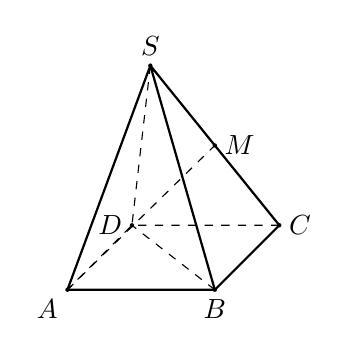
\begin{tikzpicture}[scale=.78,>=stealth]
\coordinate (A) at (0,0); \coordinate (B) at (2.4,0);
\coordinate (C) at (3.45,1.05); \coordinate (D) at (1.05,1.05);
\coordinate (S) at (1.35,3.65); \coordinate (M) at (2.40,2.35);
\draw[thick] (A)--(B)--(C);
\draw[dashed] (C)--(D)--(A) (S)--(D);
\draw[thick] (S)--(A) (S)--(B) (S)--(C);
\draw[dashed] (A)--(M) (B)--(D);
\fill (A) circle (1pt) node[below left] {$A$};
\fill (B) circle (1pt) node[below] {$B$};
\fill (C) circle (1pt) node[right] {$C$};
\fill (D) circle (1pt) node[left] {$D$};
\fill (S) circle (1pt) node[above] {$S$};
\fill (M) circle (1pt) node[right] {$M$};
\end{tikzpicture}
\end{center}
\nopagebreak[4]
（1） 证明：$M$ 是侧棱 $SC$ 的中点；

（2） 求二面角 $S-AM-B$ 的大小。

\Needspace{4\baselineskip}
\textbf{解析}

\gksubpart{(1)}

取
$A=(0,0,0)$、$B=(2,0,0)$、$D=(0,\sqrt2,0)$、$C=(2,\sqrt2,0)$、
$S=(0,\sqrt2,2)$。设 $M=S+t(C-S)$，点积公式
$\cos\angle ABM=1/2$ 化简为 $(1-t)^2=1/4$。由线段范围得
$t=1/2$，即 $M$ 为 $SC$ 中点。

\gksubpart{(2)}

\Needspace{5\baselineskip}
此时 $M=(1,\sqrt2,1)$。取

\nopagebreak[4]
\[
\boldsymbol u=\overrightarrow{MS}=(-1,0,1),
\]

\Needspace{5\baselineskip}
以及 $\overrightarrow{MB}$ 在垂直于 $AM$ 平面内的投影

\nopagebreak[4]
\[
\boldsymbol v=\overrightarrow{MB}
-\frac{\overrightarrow{MB}\cdot\overrightarrow{AM}}
{|\overrightarrow{AM}|^2}\overrightarrow{AM}
=\left(\frac32,-\frac{\sqrt2}{2},-\frac12\right).
\]

于是 $|\boldsymbol u|=\sqrt2$、$|\boldsymbol v|=\sqrt3$、
\Needspace{5\baselineskip}
$\boldsymbol u\cdot\boldsymbol v=-2$，故

\nopagebreak[4]
\[
\cos\angle(S-AM-B)=-\sqrt{\frac23}.
\]

\gkanswer{答案（1）：见解析版}

\gkanswer{答案（2）：二面角 $S-AM-B$ 的大小为 $\theta=\arccos\left(-\sqrt{\dfrac23}\right)$。}

\end{answer}
\begin{answer}
\gksolhead{19}{}

\textbf{题目}：

甲、乙二人进行一次围棋比赛，约定先胜 $3$ 局者获得这次比赛的胜利，比赛结束。假设在一局中，甲获胜的概率为 $0.6$，乙获胜的概率为 $0.4$，各局比赛结果相互独立，已知前 $2$ 局中甲、乙各胜 $1$ 局。

（1） 求甲获得这次比赛胜利的概率；

（2） 设 $\xi$ 表示从第 $3$ 局开始到比赛结束所进行的局数，求 $\xi$ 的分布列及数学期望。

\Needspace{4\baselineskip}
\textbf{解析}

\gksubpart{(1)}

\Needspace{5\baselineskip}
从第三局开始双方均还需胜两局。甲最终获胜的概率为

\nopagebreak[4]
\[
0.6^2+2(0.6)(0.4)(0.6)=\frac{81}{125}.
\]

\gksubpart{(2)}

若从第三局起两局结果相同，比赛在两局后结束；若结果一胜一负，
\Needspace{5\baselineskip}
需进行到第五局。因此

\nopagebreak[4]
\[
\Pr(\xi=2)=0.6^2+0.4^2=\frac{13}{25},\quad
\Pr(\xi=5)=2(0.6)(0.4)=\frac{12}{25},
\]

\nopagebreak[4]
\[
\mathbb E\xi=2\cdot\frac{13}{25}+5\cdot\frac{12}{25}
=\frac{86}{25}.
\]

\gkanswer{答案（1）：$\dfrac{81}{125}$}

\gkanswer{答案（2）：$\Pr(\xi=2)=\dfrac{13}{25}$，$\Pr(\xi=5)=\dfrac{12}{25}$，$\mathbb E\xi=\dfrac{86}{25}$。}

\end{answer}
\begin{answer}
\gksolhead{20}{}

\textbf{题目}：

在数列 $\{a_n\}$ 中，$a_1=1$，$a_{n+1}=\left(1+\dfrac1n\right)a_n+\dfrac{n+1}{2^n}$。

（1） 设 $b_n=\dfrac{a_n}{n}$，求数列 $\{b_n\}$ 的通项公式；

（2） 求数列 $\{a_n\}$ 的前 $n$ 项和 $S_n$。

\Needspace{4\baselineskip}
\textbf{解析}

\gksubpart{(1)}

\Needspace{5\baselineskip}
令 $b_n=a_n/n$，则

\nopagebreak[4]
\[
b_{n+1}=\frac{a_{n+1}}{n+1}
=\frac{a_n}{n}+\frac1{2^n}
=b_n+\frac1{2^n}.
\]

\gksubpart{(2)}

\Needspace{5\baselineskip}
因 $b_1=1$，故

\nopagebreak[4]
\[
b_n=1+\sum_{k=1}^{n-1}\frac1{2^k}
=2-\frac1{2^{n-1}},
\]

\Needspace{5\baselineskip}
从而

\nopagebreak[4]
\[
a_n=2n-\frac n{2^{n-1}}.
\]

\Needspace{5\baselineskip}
再由 $\sum_{k=1}^n k/2^{k-1}=4-(n+2)/2^{n-1}$，得

\nopagebreak[4]
\[
S_n=n(n+1)-4+\frac{n+2}{2^{n-1}}.
\]

\gkanswer{答案（1）：$b_n=2-2^{1-n}$。}

\gkanswer{答案（2）：$a_n=2n-\dfrac{n}{2^{n-1}}$，$S_n=n(n+1)-4+\dfrac{n+2}{2^{n-1}}$。}

\end{answer}
\begin{answer}
\gksolhead{21}{}

\textbf{题目}：

如图，已知抛物线 $E:y^2=x$ 与圆 $M:(x-4)^2+y^2=r^2$（$r>0$）相交于 $A\text{、}B\text{、}C\text{、}D$ 四个点。
\nopagebreak[4]
\begin{center}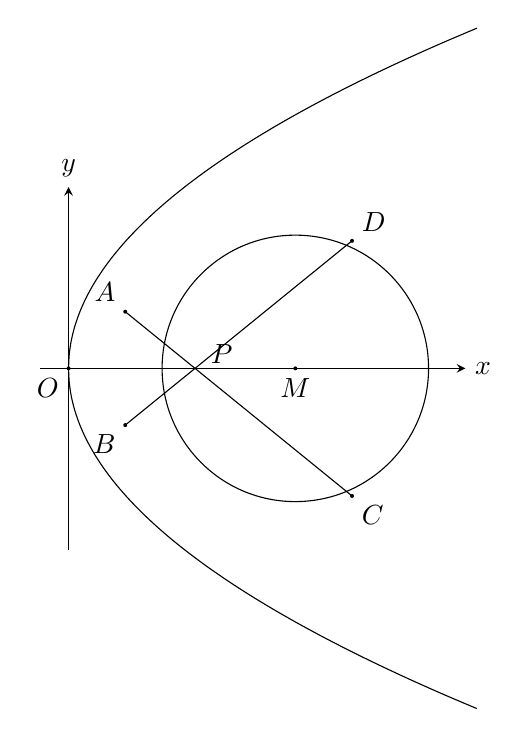
\begin{tikzpicture}[scale=.72,>=stealth]
\draw[->] (-.5,0)--(7,0) node[right] {$x$};
\draw[->] (0,-3.2)--(0,3.2) node[above] {$y$};
\draw[domain=0:6,smooth,variable=\x] plot ({\x*\x/5},{\x});
\draw[domain=0:6,smooth,variable=\x] plot ({\x*\x/5},{-\x});
\draw (4,0) circle (2.35);
\coordinate (A) at (1.0,1.0); \coordinate (B) at (1.0,-1.0);
\coordinate (C) at (5.0,-2.25); \coordinate (D) at (5.0,2.25);
\draw (A)--(C) (B)--(D);
\fill (0,0) circle (1pt) node[below left] {$O$};
\fill (4,0) circle (1pt) node[below] {$M$};
\fill (A) circle (1pt) node[above left] {$A$};
\fill (B) circle (1pt) node[below left] {$B$};
\fill (C) circle (1pt) node[below right] {$C$};
\fill (D) circle (1pt) node[above right] {$D$};
\node at (2.7,.25) {$P$};
\end{tikzpicture}
\end{center}
\nopagebreak[4]
（1） 求 $r$ 的取值范围；

（2） 当四边形 $ABCD$ 的面积最大时，求对角线 $AC\text{、}BD$ 的交点 $P$ 坐标。

\Needspace{4\baselineskip}
\textbf{解析}

\gksubpart{(1)}

\Needspace{5\baselineskip}
令 $t=y^2$，由 $x=y^2$ 得

\nopagebreak[4]
\[
t^2-7t+16-r^2=0.
\]

四个不同交点要求两个不同正根，故
$4r^2-15>0$ 且 $16-r^2>0$，即
$\dfrac{\sqrt{15}}2<r<4$。

\gksubpart{(2)}

设两根平方根为 $u\text{、}v$，则 $u^2+v^2=7$，四边形面积
$S=(v^2-u^2)(u+v)$。令 $z=(u+v)^2$，有
\Needspace{5\baselineskip}
$S=z\sqrt{14-z}$，在 $z=28/3$ 时最大。于是

\nopagebreak[4]
\[
uv=\frac{z-7}{2}=\frac76.
\]

对角线交点在 $x$ 轴上且横坐标为 $uv$，故
$P\left(\dfrac76,0\right)$。

\gkanswer{答案（1）：$\dfrac{\sqrt{15}}2<r<4$。}

\gkanswer{答案（2）：$P\left(\dfrac76,0\right)$。}

\end{answer}
\begin{answer}
\gksolhead{22}{}

\textbf{题目}：

设函数 $f(x)=x^3+3bx^2+3cx$ 在两个极值点 $x_1\text{、}x_2$，且 $x_1\in[-1,0]$，$x_2\in[1,2]$。
\nopagebreak[4]
\begin{center}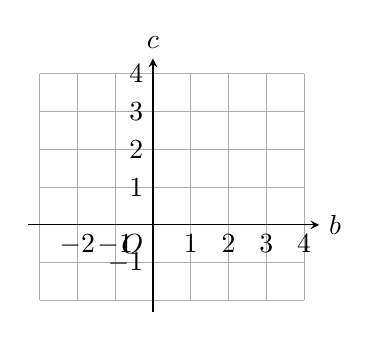
\begin{tikzpicture}[scale=.48,>=stealth]
\draw[step=1,gray!65] (-3,-2) grid (4,4);
\draw[->] (-3.3,0)--(4.4,0) node[right] {$b$};
\draw[->] (0,-2.3)--(0,4.4) node[above] {$c$};
\foreach \x in {-2,-1,1,2,3,4}
  \node[below] at (\x,0) {$\x$};
\foreach \y in {-1,1,2,3,4}
  \node[left] at (0,\y) {$\y$};
\node[below left] at (0,0) {$O$};
\end{tikzpicture}
\end{center}
\nopagebreak[4]
（1） 求 $b\text{、}c$ 满足的约束条件，并在下面的坐标平面内，画出满足这些条件的点 $(b,c)$ 的区域；

（2） 证明：$-10\leqslant f(x_2)\leqslant-\dfrac12$。

\Needspace{4\baselineskip}
\textbf{解析}

\gksubpart{(1)}

\nopagebreak[4]
\[
f'(x)=3(x^2+2bx+c),
\]

\Needspace{5\baselineskip}
其两个根就是 $x_1\text{、}x_2$，所以

\nopagebreak[4]
\[
b=-\frac{x_1+x_2}{2},\qquad c=x_1x_2,\qquad
-1\leqslant x_1\leqslant0,\quad1\leqslant x_2\leqslant2.
\]

这也给出 $(b,c)$ 区域的参数表示；边界分别来自
$x_1=-1,0$ 与 $x_2=1,2$。

\gksubpart{(2)}

令 $x_1=u$、$x_2=v$。由 $v$ 为导数的根，
\Needspace{5\baselineskip}
$c=-v^2-2bv$，代入 $f(v)$ 得

\nopagebreak[4]
\[
f(v)=\frac{v^2}{2}(3u-v).
\]

在 $-1\leqslant u\leqslant0$、$1\leqslant v\leqslant2$ 上，
$f(v)$ 的最大值为 $-1/2$（$u=0,v=1$），最小值为 $-10$
\Needspace{5\baselineskip}
（$u=-1,v=2$），故

\nopagebreak[4]
\[
-10\leqslant f(x_2)\leqslant-\frac12.
\]

\gkanswer{答案（1）：存在 $x_1\in[-1,0]$、$x_2\in[1,2]$，使 $b=-\dfrac{x_1+x_2}{2}$、$c=x_1x_2$；等价地，$(b,c)$ 是该参数变换下矩形 $[-1,0]\times[1,2]$ 的像。}

\gkanswer{答案（2）：$-10\leqslant f(x_2)\leqslant-\dfrac12$。}

\end{answer}